\documentclass[class=report,crop=false, 12pt]{standalone}
\usepackage[screen,nosolutions]{../myscratch}
%\usepackage[print]{../myscratch}



\begin{document}

\titre[S]{Si ... alors ... sinon ...}
%===============================

\insertvideo{nVhnbm-irjw}{Si ... alors ... sinon ... -- Activité 1}

\insertvideo{O4MQnGwgqjM}{Si ... alors ... sinon ... -- Activité 2}

\insertvideo{wwNLx33Subk}{Si ... alors ... sinon ... -- Activité 3}

\bigskip
\bigskip

\begin{activite}

Programme un petit quiz.

\begin{itemize}
  \item Pose une question en proposant trois réponses possibles. 
  \item L'utilisateur répond 1, 2 ou 3.
  \item Informe l'utilisateur s'il a donné ou non la bonne réponse.
\end{itemize}



\begin{center}
  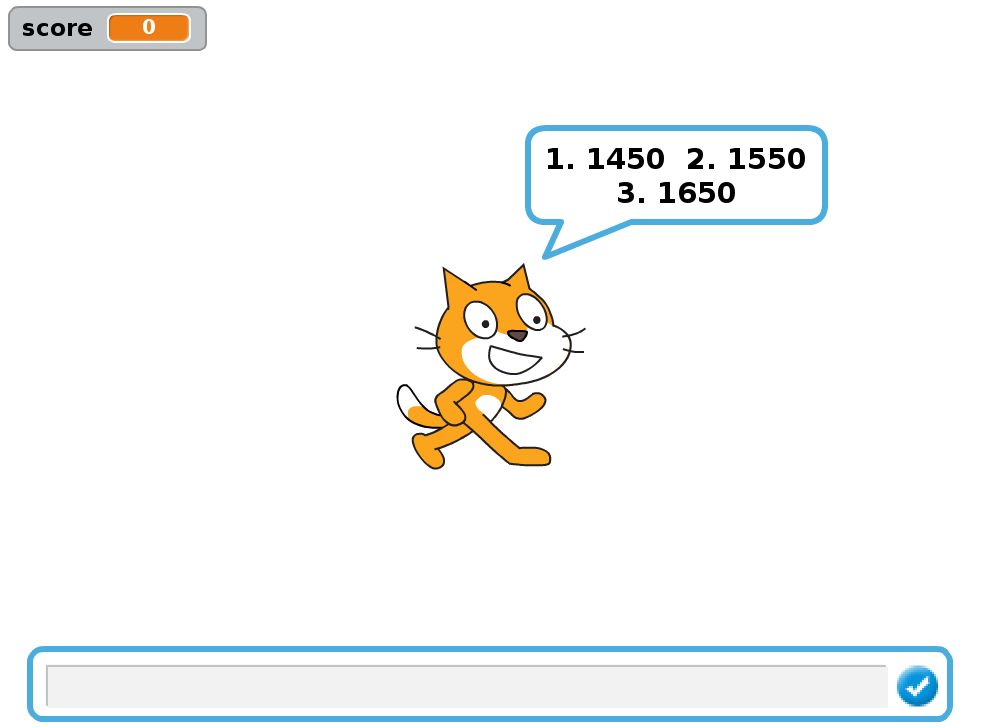
\includegraphics[width=0.95\textwidth]{ecran-07-ex1} 
\end{center}


\bigskip

\textbf{Blocs utiles.}

\begin{center}
\begin{scratch}
\blockifelse{si \boolempty{} alors}
  {\blockspace}
  {\blockspace}
\end{scratch}
\end{center} 
  
  
Exemples de questions sur le thème \og dates de l'histoire des sciences \fg{} :
\begin{itemize}
  \item L'invention de l'imprimerie (1. 1450, 2. 1550, 3. 1650).
  \item L'encyclopédie de Diderot (1. 1650, 2. 1750, 3. 1850).
  \item Second voyage de Christophe Colomb (1. 1493, 2. 1497, 3. 1502).
  \item Premier homme dans l'espace, Youri Gagarine (1. 1941, 2. 1951, 3. 1961).
  \item Premier homme sur la lune, Neil Armstrong (1. 1959, 2. 1969, 3. 1979).
  \item Premier ordinateur électronique, ENIAC (1. 1947, 2. 1967, 3. 1987).
  \item \ldots
\end{itemize} 

\medskip

\textbf{Bonus.} Tu peux poser plusieurs questions à la suite et afficher le score de l'utilisateur.

\end{activite}



\begin{activite}

Demande à l'utilisateur un nombre entre $100$ et $999$ et fais en sorte que l'ordinateur réponde si ce nombre est divisible par $5$, puis s'il est divisible par $3$.

\begin{center}
  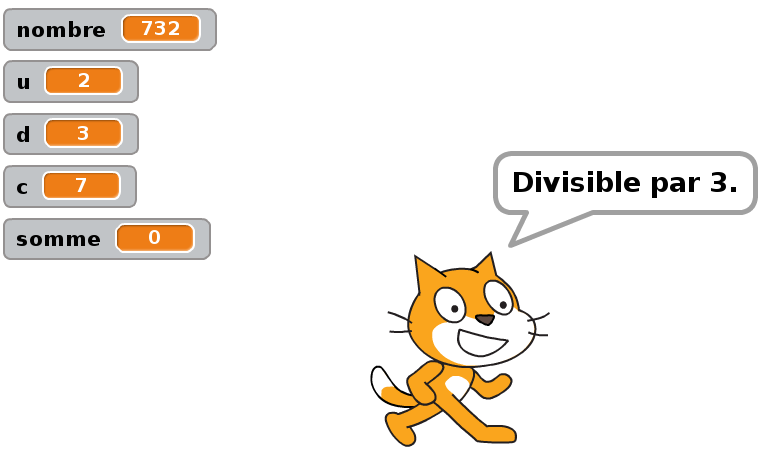
\includegraphics[width=0.6\textwidth]{ecran-07-ex2} 
\end{center}


\begin{itemize}
  \item \textbf{Critère de divisibilité par 5.}
  
  Un entier est divisible par $5$ exactement lorsque son chiffre des unités est $0$ ou $5$.
  
  Exemple : $160$ et $485$ sont divisibles par $5$, par contre $753$ ne l'est pas !
  
  \item \textbf{Critère de divisibilité par 3.}  
  
  Un entier est divisible par $3$ exactement lorsque la somme de ses chiffres est divisible par $3$.
  Exemple : $561$ est divisible par $3$, car $5+6+1=12$ est divisible par $3$.
  Par contre $917$ ne l'est pas.  
\end{itemize}

\bigskip

\textbf{Blocs utiles.}
Comment récupérer les chiffres d'un nombre ? Si ce nombre est un 
nombre à $3$ chiffres, alors on considère ce nombre comme un mot de $3$ lettres.
Par exemple, si le nombre est $492$, alors la première lettre est $4$, la deuxième est $9$, la troisième est $2$.

\begin{center}
\ovaloperator{lettre \ovalnum{1} de \ovalvariable{nombre}}

\medskip

\ovaloperator{lettre \ovalnum{2} de \ovalvariable{nombre}}

\medskip

\ovaloperator{lettre \ovalnum{3} de \ovalvariable{nombre}}

\end{center} 




\end{activite}



\begin{activite}

Programme un jeu de calcul mental.

\begin{center}
  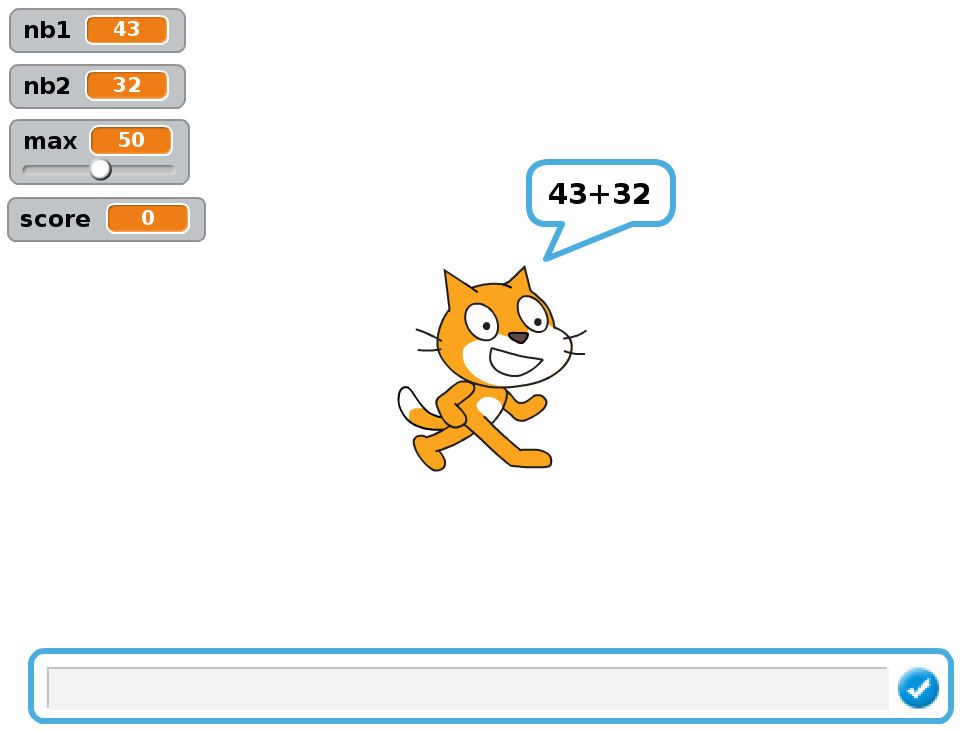
\includegraphics[width=0.89\textwidth]{ecran-07-ex3} 
\end{center}

\begin{itemize}
  \item Fixe un maximum (par exemple $50$).
  \item Tire deux nombres au hasard plus petits que ce maximum.
  \item Demande combien vaut la somme de ces deux nombres.
  \item Vérifie le résultat. Si la réponse est juste, augmente le score du joueur, sinon joue un son.
  \item Demande plusieurs calculs et affiche le score final.
\end{itemize}

\end{activite}



\ifx \displaysolutions \myzero
\else
\begin{code}
\setscratch{scale=0.45}
\onesolution{Si ... alors ... sinon ...}{Activité 1}{
  \begin{minipage}{0.45\textwidth}
    \begin{scratch}
      \blockinit{quand \greenflag est cliqué}
      \blockvariable{mettre \selectmenu{score} à \ovalnum{0}}
      \blocklook{dire \ovalnum{Date de l'invention de l'imprimerie ?} pendant \ovalnum{2} secondes}
      \blocksensing{demander \ovalnum{1. 1450 2. 1550 3. 1650} et attendre}
      \blockifelse{si \booloperator{\ovalsensing{réponse} = \ovalnum{1}} alors }
                  {
                    \blockvariable{ajouter \ovalnum{1} à \selectmenu{score}}
                    \blocklook{dire \ovalnum{Bravo !} pendant \ovalnum{2} secondes}
                  }
                  {
                    \blocklook{dire \ovalnum{Mauvaise réponse !} pendant \ovalnum{2} secondes}
                  }


      \blocklook{dire \ovaloperator{regrouper \ovalnum{Score =} et \ovalvariable{score}}}
      \blocklook{dire \ovalnum{Date de la publication de L'encyclopédie de Diderot ?} pendant \ovalnum{2} secondes}
      \blocksensing{demander \ovalnum{1. 1650, 2. 1750, 3. 1850} et attendre} 
    \end{scratch}
    \medskip
    \mbox{$\vdots$}
  \end{minipage}
}
\onesolution{Si ... alors ... sinon ...}{Activité 2}{
\begin{scratch}
  \blockinit{quand \greenflag est cliqué}
  \blocksensing{demander \ovalnum{Choisis un nombre entre 100 et 999 !} et attendre}
  \blockvariable{mettre \selectmenu{nombre} à \ovalsensing{réponse}}
  \blockvariable{mettre \selectmenu{u} à \ovaloperator{lettre \ovalnum{3} de \ovalvariable{nombre}}}
  \blockvariable{mettre \selectmenu{d} à \ovaloperator{lettre \ovalnum{2} de \ovalvariable{nombre}}}
  \blockvariable{mettre \selectmenu{c} à \ovaloperator{lettre \ovalnum{1} de \ovalvariable{nombre}}}
  \blockifelse{si \booloperator{\booloperator{\ovalvariable{u} = \ovalnum{0}} ou \booloperator{\ovalvariable{u} = \ovalnum{5}}} alors }
  {
    \blocklook{dire \ovalnum{Divisible par 5} pendant \ovalnum{2} secondes}
  }
  {
    \blocklook{dire \ovalnum{Pas divisible par 5} pendant \ovalnum{2} secondes}
  }
  \blockvariable{mettre \selectmenu{somme} à  
     \ovaloperator{\ovalvariable{u} + \ovaloperator{\ovalvariable{d} + \ovalvariable{c}}} 
  }
  \blockrepeat{répéter jusqu'à ce que 
    \booloperator{\ovalvariable{somme} < \ovalnum{3}}}
  {
    \blockvariable{ajouter \ovalnum{-3} à \selectmenu{somme}}
  }
  \blockifelse{si \booloperator{\ovalvariable{somme} = \ovalnum{0}} alors }
  {
    \blocklook{dire \ovalnum{Et divisible par 3} pendant \ovalnum{2} secondes}
  }
  {
    \blocklook{dire \ovalnum{Et pas divisible par 3} pendant \ovalnum{2} secondes}
  }
\end{scratch}
}
\onesolution{Si ... alors ... sinon ...}{Activité 3}{
\begin{scratch}
  \blockinit{quand \greenflag est cliqué}
  \blockvariable{mettre \selectmenu{max} à \ovalnum{50}}
  \blockvariable{mettre \selectmenu{score} à \ovalnum{0}}
  \blockrepeat{répéter \ovalnum{3} fois}
  {
    \blockvariable{mettre \selectmenu{nb1} à \ovaloperator{nombre aléatoire entre \ovalnum{1} et \ovalvariable{max}}}
    \blockvariable{mettre \selectmenu{nb2} à \ovaloperator{nombre aléatoire entre \ovalnum{1} et \ovalvariable{max}}}
    \blocksensing{demander 
      \ovaloperator{regrouper 
        \ovaloperator{regrouper \ovalvariable{nb1} et \ovalnum{+}}
        et \ovalvariable{nb2}}
      et attendre} 
    \blockifelse{si \booloperator{\ovalsensing{réponse} = \ovaloperator{\ovalvariable{nb1} + \ovalvariable{nb2} }} alors }
    {
      \blockvariable{ajouter \ovalnum{1} à \selectmenu{score}}
    }
    {
      \blocksound{jouer le son \ovalsound*{miaou}}
    }
  }
  \blocklook{dire \ovaloperator{regrouper \ovalnum{Score =} et \ovalvariable{score}}}
\end{scratch}
}    
\end{code}
\fi

\end{document}

